\documentclass[letterpaper,10pt,onecolumn,draftclsnofoot]{IEEEtran}
\usepackage{times}

\usepackage[english]{babel}
\usepackage[margin=0.75in]{geometry}

\usepackage{graphicx}
\DeclareGraphicsExtensions{.pdf,.png,.jpg}

\title{Object speed Tracking}
\author{Alex Bailey, Ben Wick, Dylan WashburneCS 461, Fall Term}

\begin{document}

\begin{titlepage}

\maketitle

\begin{abstract}
Using a stationary camera, with the intent of being mounted on a car, we are attempting to  detect objects and determine the speeds of those objects relative to the Observer (camera).
This will be done by having the camera recognize objects in space and determine their speeds based on the rate at which they travel through the frame.
If the camera is on a moving object, then we will need to either have a way for the system to measure it's own speed, likely with an accelerometer or connect to the object, if the object is measuring it's own speed.
To make this work, we will have to research the varieties of cameras available to use, as well as the API’s  they operate with.
We will also have to review the available computer vision algorithms and determine which is the most appropriate.
From this, we will determine the best camera to be used and from there create a object tracking program.
 
\end{abstract}

\end{titlepage}

\section{Problem Definition}

There are many applications for tracking the speeds of moving objects.
One example is tracking the speed of a vehicle for use by police enforcing speed limits.
 Current methods for tracking the speed of an object include radar guns and laser scanners, however, speed tracking methods like this include various problems.

 Primary among these problems is that radar and similar methods perform poorly in poor weather conditions.
 Plus the methods that require radar and laser put out a detectable signal that the object being tracked can detect.
  Methods like these are also only capable of tracking one object at a time.
 In our modern society, these shortcomings are no longer acceptable.
 We have used the methods provided to us because there were no other options to work with.


%Distance is maybe an issue to look for

\section{Proposed Solution}

We are going to use a camera and a computer vision program to identify objects and to track the speed of passing objects.
 The system will be able to track passing objects and display their current speeds to the user.
 The system will also be able to accurately detect the speeds of passing objects during inclement weather conditions, such as heavy rain, in which other methods would return bad results.
 The camera and computer vision system to be used is yet to be determined, however we can select the camera and computer vision system to use by examining the strengths and shortcomings presented.
 After selecting a camera and computer vision system, we will work to incorporate the computer vision system with the camera’s api to determine object recognition.
 From there, we will gauge the object’s speed based on its movement in-frame, so that we can return instantaneous results to the user.
 

\section{Performance Metrics}

Our solution will be able to identify and detect nearby objects which can be tracked.
 The system will then track the nearby object to determine speed, and return the value within 10\% of its actual speed.
 If possible, the solution will also be able to perform this on multiple objects simultaneously.
 We will also work to make the results displayed to the user appear instantaneously, with as little required lag as possible.

 
%Applications somewhere maybe

\hfill \break
\hfill \break
\hfill \break

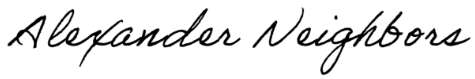
\includegraphics[scale=0.5]{signature}


\end{document}